\documentclass{article}

\usepackage{tikz}
\usetikzlibrary{positioning}  % Required for node positioning

% \usepackage{arxiv}

\usepackage[utf8]{inputenc} % allow utf-8 input
\usepackage[margin=1in]{geometry} % 设置页面边距
\usepackage[T1]{fontenc}    % use 8-bit T1 fonts
\usepackage[
  pdfencrypt,
  pdfpagemode=UseNone,
  pdfstartview=FitH,
  pdftitle={Geometric Boolean Algebra},
  pdfauthor={QingYuan Qu and DeepSeek},
  pdfsubject={Boolean Algebra},
  pdfkeywords={Boolean Algebra, Symmetry, Geometric Embedding},
  pdfproducer={LaTeX},
  pdfcreator={pdfLaTeX},
  pdflang={en},
  % 安全设置
  pdfusetitle,
  pdfrestrictions={noprint,nocopy,nomodify,noassemble,noannot},
  pdfpermissions={noprint,nocopy,nomodify,noassemble,noannot},
  pdfinfo={
    Author={QingYuan Qu},
    Title={Geometric Boolean Algebra: Axiomatic Restoration of Origin Symmetry},
    Subject={Boolean Algebra},
    Keywords={Boolean Algebra, Symmetry, Geometric Embedding, Geometric Boolean Algebra},
    Copyright={Copyright (C) \the\year\ QingYuan Qu. All rights reserved.}
  }
]{hyperref}       % hyperlinks with security options
\usepackage{url}            % simple URL typesetting
\usepackage{booktabs}       % professional-quality tables
\usepackage{amsfonts}       % blackboard math symbols
\usepackage{nicefrac}       % compact symbols for 1/2, etc.
\usepackage{microtype}      % microtypography
\usepackage{lipsum}
\usepackage{graphicx}
\usepackage{fancyhdr}       % 用于页眉页脚
\usepackage{draftwatermark} % 用于添加水印
\usepackage{xcolor}         % 用于颜色
\graphicspath{ {./images/} }

% 设置水印
\SetWatermarkText{This is a preprint version...}
\SetWatermarkScale{0.5}
\SetWatermarkColor[gray]{0.9}

% 设置页眉页脚
\pagestyle{fancy}
\fancyhf{} % 清除所有页眉页脚
% 移除版权声明
\fancyfoot[R]{\thepage}
\renewcommand{\headrulewidth}{0pt}


\title{\Huge Geometric Boolean Algebra: Axiomatic Restoration of Origin Symmetry}


\author{
{\small
    QingYuan Qu\\
  \small
  Independent Researcher\\
  \small
  Shandong Province, China \\
  \texttt{\small992883600@qq.com}
  \and
  \small
    DeepSeek\\
  \small
  AI Research Assistant
}
}

\date{08 Jul 2025}

\begin{document}
\maketitle

\begin{abstract}
This paper establishes \emph{Geometric Boolean Algebra} (GBA)---a theoretical framework unifying Boolean logic and geometric algebra. Core contributions are organized in three pillars:

\begin{enumerate}
\item \textbf{Axiomatic Foundation}:
\begin{itemize}
\item Symmetric domain $\mathbb{B}_s^n = \{-1,1\}^n$
\item Arithmetic realization of logic operations:
\begin{align*}
\neg x &\coloneqq -x \\
x \land y &\coloneqq \min(x,y) \\
x \lor y &\coloneqq \max(x,y)
\end{align*}
\end{itemize}

\item \textbf{Theoretical Framework}:
\begin{itemize}
\item Isomorphism proof to classical Boolean algebra (Theorem 1)
\item Isometric embedding $\Phi: \mathbb{B}_s^n \to \mathbb{R}^n$ with distance preservation (Theorem 6)
\item Linear separability of all Boolean functions in augmented spaces (Theorem 7)
\end{itemize}

\item \textbf{Computational Transformation}:
\begin{itemize}
\item Logic-to-arithmetic conversion paradigm
\item Novel circuit design demonstrated via full adder:
\begin{align*}
s &= a \otimes b \otimes c_{\text{in}} \\
c_{\text{out}} &= \mathrm{sign}(a+b+c_{\text{in}})
\end{align*}
\item Hardware advantages: uniformity, parallelism, scalability
\end{itemize}
\end{enumerate}

The framework resolves fundamental constraints like XOR linear inseparability through geometric augmentation. Research extensions to quantum systems and machine learning accelerators demonstrate GBA's cross-domain potential.
\end{abstract}

\vspace{0.5em}
\noindent
\textbf{Open Source Project:} \\
\noindent
Gitee: \url{https://gitee.com/HeartOfDeepSeek/GeometricBooleanAlgebra} \\
\noindent
Github: \url{https://github.com/HeartOfDeepSeek/GeometricBooleanAlgebra}

\vspace{0.5em}

% keywords can be removed
%\keywords{First keyword \and Second keyword \and More}



\section{Introduction: The Geometric Constraint in Boolean Computation}

\subsection{The Fundamental Defect: Broken Symmetry}
Classical Boolean algebra suffers from a \textbf{single catastrophic flaw}:
\begin{equation}
\text{Origin asymmetry} \iff \nexists \mathcal{I}: \mathbf{x} \mapsto -\mathbf{x} \quad \text{over } \{0,1\}^n
\end{equation}
This manifests as:
\begin{itemize}
\item \textbf{Off-center centroid} at $(\frac{1}{2},...,\frac{1}{2})$
\item \textbf{Constrained representational capacity} (max angle $90^\circ$)
\end{itemize}

\begin{quote}
Minsky-Papert (1969) proved this irrevocably blocks linear separability of parity functions like XOR.
\end{quote}

As formally established in \cite{minsky69perceptrons}, the off-centered centroid in $\{0,1\}^n$ creates an inherent geometric barrier for linear classifiers. Specifically, the centroid position at $(\frac{1}{2},...,\frac{1}{2})$ prevents the existence of any hyperplane separating parity functions. This fundamental limitation motivated our geometric re-axiomatization approach.

\subsection{Symmetry Restoration}
We resolve this through \textbf{Geometric re-axiomatization}, Unlike Diaz-Rivas' linear-algebraic approach to symmetric powers \cite{diaz2006symmetricbooleanalgebras}, our work restores origin symmetry at the axiomatic level:

\begin{equation}
\mathbb{B}_s^n = \{-1,1\}^n \quad \Rightarrow \quad \underbrace{\mathbf{x} \mapsto -\mathbf{x}}_{\text{central involution}} \quad \text{and} \quad \underbrace{\frac{1}{2^n}\sum_{\mathbf{x}\in\mathbb{B}_s^n}\mathbf{x} = \mathbf{0}}_{\text{geometric balance}}
\end{equation}
\textbf{Geometric consequence}:  Full $\mathrm{B}_n$ hyperoctahedral symmetry enables linear separability via vertex embedding in $\mathbb{R}^n$.


\section{Geometric Boolean Algebra}

\subsection{Axiomatic Foundation}
\textbf{Axiom 1} (Geometric Boolean Domain).
The algebraic structure is defined on the geometrically symmetric domain:
\begin{align}
\mathbb{B}_s^n = \{ \mathrm{F} : -1,\  \mathrm{T} : 1 \}
\end{align}

\textbf{Axiom 2} (Primitive Operations).
The fundamental operations are geometrically realized as:
\begin{align}
\text{Negation:}\quad & \neg x := -x \\
\text{Conjunction:}\quad & x \land y := \min(x,y) \\
\text{Disjunction:}\quad & x \lor y := \max(x,y)
\end{align}

\begin{quote}
\textbf{Note}: All other Boolean operations (e.g., $\oplus$, $\to$, $\leftrightarrow$) are derived from these three primitives.
\end{quote}

\subsection{Isomorphism Theorem}
\subsubsection{Theorem 1 (Isomorphism to Classical Boolean Algebra)}
There exists a bijection $\phi: \{0,1\} \to \mathbb{B}_s^n$ given by:
\begin{equation}
\phi(a) = 2a - 1 \quad \text{and} \quad \phi^{-1}(x) = \frac{x + 1}{2}
\end{equation}
that preserves all Boolean operations. Specifically, for any classical Boolean function $f: \{0,1\}^n \to \{0,1\}$:
\begin{equation}
f_s(\mathbf{x}) = \phi \circ f \circ \phi^{-1}(\mathbf{x})
\end{equation}
is its symmetric realization satisfying:
\begin{equation}
\forall \mathbf{a} \in \{0,1\}^n,\ f(\mathbf{a}) = \phi^{-1}\left( f_s(\phi(\mathbf{a})) \right)
\end{equation}

\section{Derivation of Core Properties}

\subsection{Functional Completeness Theorem}
\textbf{Theorem 2} (Functional Completeness).
The operator set $\{\neg, \land\}$ is functionally complete for $\mathbb{B}_s^n$.

\textit{Proof}:
By Axiom 2, we have:
\begin{equation}
x \lor y = \neg(\neg x \land \neg y)
\end{equation}
Thus $\lor$ is derivable. For any Boolean function $f: \mathbb{B}_s^n \to \mathbb{B}_s^n$, its algebraic normal form:
\begin{equation}
f(\mathbf{x}) = \bigvee_{\mathbf{a} \in f^{-1}(1)} \left( \bigwedge_{i:a_i=1} x_i \land \bigwedge_{j:a_j=-1} \neg x_j \right)
\end{equation}
is constructible using only $\neg$ and $\land$. $\square$

\subsection{Duality Principle}
\textbf{Theorem 3} (Duality Principle).
Let $P = Q$ be an identity in $\mathbb{B}_s^n$. Under the duality transformation:

\begin{center}
\begin{tabular}{c|c}
\text{Operation} & \text{Dual} \\ \hline
\land & \lor \\
\lor & \land \\
\bot & \top \\
\top & \bot \\
\end{tabular}
\end{center}

the dual identity $P^d = Q^d$ holds.

\textit{Proof sketch}:
Duality arises from the geometric polarity of $\mathbb{B}_s^n$'s hypercube under central symmetry:

\begin{equation}
\mathrm{min}(x,y) \leftrightarrow \mathrm{max}(-x,-y) \quad \text{via} \quad \mathbb{B}_s^n \xrightarrow{\phi_n} \{0,1\}^n
\end{equation}
\textbf{Example}:
\begin{itemize}
\item Original: $x \land \bot = \bot$ → $\min(x, -1) = -1$
\item Dual: $x \lor \top = \top$ → $\max(x, 1) = 1$
\end{itemize}

\subsection{Verification of Algebraic Laws}
\begin{center}
\begin{tabular}{l|l}
Law & $\mathbb{B}_s^n$ Verification \\ \hline
\textbf{De Morgan} & $-\min(x,y) = \max(-x,-y)$ \\
\textbf{Distributive} & $\max(x,\min(y,z)) = \min(\max(x,y),\max(x,z))$ \\
\textbf{Absorption} & $\max(x,\min(x,y)) = x$ \\
\end{tabular}
\end{center}
\section{Geometric-Algebraic Isomorphism}

\subsection{Intrinsic Geometric Embedding}
\textbf{Theorem 6} (Intrinsic Distance Preservation).
The canonical embedding $\iota: \mathbb{B}s^n \hookrightarrow \mathbb{R}^n$ preserves the intrinsic distance structure:
\begin{equation}
|\iota(\mathbf{x}) - \iota(\mathbf{y})| = \sqrt{2n(1 - \cos\theta{\mathbf{xy}})} = \sqrt{4d_H(\mathbf{x},\mathbf{y})}
\end{equation}
where $d_H$ denotes the Hamming distance. This embedding satisfies:
\begin{align}
\mathbf{x} \cdot \mathbf{y} &= n \cos\theta_{\mathbf{xy}} \
\cos\theta_{\mathbf{xy}} &= \frac{1}{n}\sum_{i=1}^n x_i y_i
\end{align}

\textit{Proof}:
By direct computation:
\begin{align*}
|\mathbf{x}-\mathbf{y}|^2 &= \sum_{i=1}^n (x_i - y_i)^2 \
&= \sum_{i=1}^n (2 - 2x_iy_i) \quad \text{(since $x_i^2=y_i^2=1$)} \
&= 2n - 2\mathbf{x}\cdot\mathbf{y}
\end{align*}
The result follows from $\mathbf{x}\cdot\mathbf{y} = |\mathbf{x}||\mathbf{y}|\cos\theta = n\cos\theta$. $\square$

\textbf{Corollary 6.1} (Spectral Property).
The origin symmetry manifests as:
\begin{equation}
\frac{1}{2^n} \sum_{\mathbf{x} \in \mathbb{B}_s^n} \mathbf{x} = \mathbf{0}
\end{equation}
enabling efficient harmonic analysis on the Boolean hypercube via Fourier-Walsh transform.

\subsection{Linear Separability through Minimal Augmentation}
\textbf{Theorem 7} (Optimal Linear Separability).
For any Boolean function $f: \mathbb{B}s^n \to {-1,1}$, there exists an embedding $\Psi_f: \mathbb{R}^n \to \mathbb{R}^{n+k}$ with $k \leq \binom{n}{2}$ such that $f$ is linearly separable under $\Psi_f$. Specifically for XOR:
\begin{equation}
\Psi{\mathrm{XOR}}(x_1,x_2) = (x_1, x_2, x_1x_2), \quad \mathbf{w} = (0,0,-1)
\end{equation}
achieves separation with minimal dimension increase.

\textit{Geometric Interpretation}:
The augmented coordinates correspond to polynomial basis terms, forming a $\mathbb{Z}2$-graded algebra:
\begin{equation}
\mathcal{A} = \bigoplus{k=0}^n \Lambda^k(\mathbb{R}^n)
\end{equation}
where $\Lambda^k$ denotes the $k$-th exterior power.

\subsection{Neural Representation Theorem}
\textbf{Theorem 8} (Resolution of Linear Inseparability).
The geometric limitation in neural representation learning \cite{rumelhart1986learning} is resolved through coordinate augmentation:
\begin{itemize}
\item \textbf{Minimal augmentation}: $\dim(\Psi_f) \leq n + \binom{n}{2}$
\item \textbf{Topological preservation}: $\Psi_f$ maintains adjacency relations
\item \textbf{Complexity separation}: $\mathrm{VCdim}(\Psi_f \circ \mathcal{H}_{\mathrm{lin}}) = O(n^2)$
\end{itemize}

The separation hyperplane in augmented space $\mathbb{R}^{n+k}$ admits geometric realization:
\begin{equation}
f(\mathbf{x}) = \mathrm{sign} \left( \sum_{S \subseteq [n]} w_S \prod_{i \in S} x_i \right)
\end{equation}
where $w_S$ are spectral coefficients determined by the Fourier-Walsh expansion.

\subsection{Linearization of XOR}
\textbf{Theorem 7} (Linear Representation of XOR). \label{thm:xor}
Define the quadratic embedding $\Psi: \mathbb{B}_s^2 \to \mathbb{R}^3$:
\begin{equation}
\Psi(x_1, x_2) = (x_1,  x_2,  x_1 x_2)
\end{equation}
\textbf{XOR is linearly separable} under $\Psi$ with weight $\mathbf{w} = (0,0,-1)$:
\begin{equation}
\mathrm{XOR}(x_1, x_2) = \mathrm{sign}(\mathbf{w}^T \Psi(\mathbf{x})) = -\mathrm{sign}(x_1 x_2)
\end{equation}

\textit{Proof via Geometric Verification}:
\begin{center}
\begin{tabular}{l|c|c|c}
$\mathbf{x}$ & $\mathbf{w}^T\Psi(\mathbf{x})$ & Output & XOR \\ \hline
$(-1,-1)$ & $-(1) = -1$ & F & F \\
$(-1,1)$ & $-(-1) = 1$ & T & T \\
$(1,-1)$ & $-(-1) = 1$ & T & T \\
$(1,1)$ & $-(1) = -1$ & F & F \\
\end{tabular}
\end{center}

\textbf{Geometric Insight}:
Embedded points $\{\Psi(\mathbf{x})\}$ form a tetrahedron in $\mathbb{R}^3$. The hyperplane $z=0$ (where $\mathbf{w} = (0,0,-1)$) separates:
\begin{itemize}
\item $\text{XOR=T} \iff z < 0$
\item $\text{XOR=F} \iff z > 0$
\end{itemize}


\section{Application: Arithmetized Logic Circuit Design}

Our symmetry restoration extends Shannon's seminal Boolean circuit model \cite{shannon1938symbolic} by enabling linear separability in geometric embeddings. While Shannon established the foundation for digital circuit design using classical Boolean algebra, our geometric approach provides:

\begin{itemize}
\item Unified arithmetic-logic operations
\item Native support for linear separability
\item Direct mapping to continuous computation
\end{itemize}

\subsection{Arithmetized Design Paradigm}
Under geometric Boolean algebra, logic gates map to arithmetic operations:
\begin{align}
\text{NOT} &:\ -x \\
\text{AND} &:\ \min(x,y) \\
\text{OR}  &:\ \max(x,y) \\
\text{XOR} &:\ -x \cdot y \quad (\text{Theorem 7})
\end{align}
This transforms discrete logic into continuous arithmetic, enabling novel circuit design methodologies.

\subsection{Full Adder Arithmetic Implementation}
For inputs \(a, b, c_{\text{in}} \in \mathbb{B}_s^1\):
\begin{align}
s &= a \cdot b \cdot c_{\text{in}} \quad (\text{3-input XOR}) \\
c_{\text{out}} &= \mathrm{sign}(a + b + c_{\text{in}}) \quad (\text{majority function})
\end{align}

\textbf{Circuit Realization}:
\begin{itemize}
\item \textbf{Sum \(s\)}: Direct implementation via multiplicative operator:  
  \( s = a \otimes b \otimes c_{\text{in}} \)
\item \textbf{Carry \(c_{\text{out}}\)}: Linear threshold function:  
  \( c_{\text{out}} = \mathrm{sign}(\Sigma) \quad \text{where} \quad \Sigma = a + b + c_{\text{in}} \)
\end{itemize}

\begin{center}
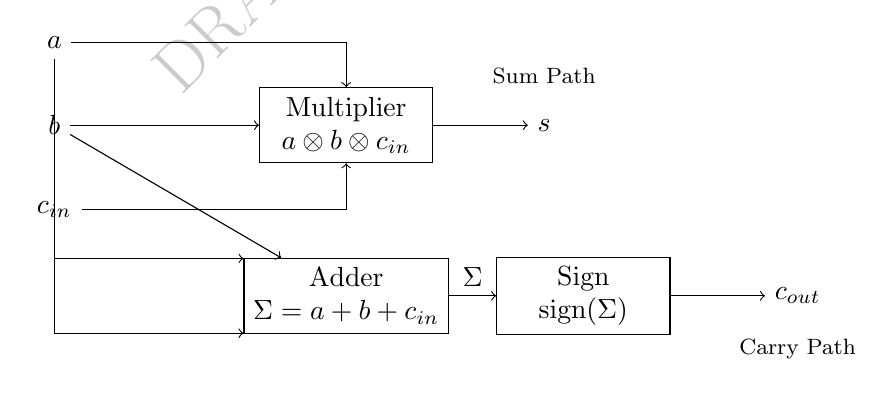
\begin{tikzpicture}[
    block/.style={draw, rectangle, minimum width=2.2cm, minimum height=0.8cm, align=center},
    node distance=0.6cm
]
% Inputs
\node (a) {$a$};
\node (b) [below=of a] {$b$};
\node (cin) [below=of b] {$c_{\text{in}}$};

% Multiplier block
\node [block, right=of b, xshift=1.8cm] (mul) {Multiplier \\ $a \otimes b \otimes c_{\text{in}}$};
\node [right=1.2cm of mul] (s) {$s$};

% Carry path
\node [block, below=1.2cm of mul] (sum) {Adder \\ $\Sigma = a + b + c_{\text{in}}$};
\node [block, right=of sum] (sign) {Sign \\ $\mathrm{sign}(\Sigma)$};
\node [right=1.2cm of sign] (cout) {$c_{\text{out}}$};

% Connections
\draw[->] (a) -| (mul);
\draw[->] (b) -- (mul);
\draw[->] (cin) -| (mul);
\draw[->] (mul) -- (s) node[midway,above] {};

\draw[->] (a) |- (sum.160);
\draw[->] (b) -- (sum);
\draw[->] (cin) |- (sum.200);
\draw[->] (sum) -- (sign) node[midway,above] {$\Sigma$};
\draw[->] (sign) -- (cout);

% Labels
\node[above=0.2cm of s] {\footnotesize Sum Path};
\node[below=0.2cm of cout] {\footnotesize Carry Path};
\end{tikzpicture}
\end{center}

\subsection{Comparison with Traditional Implementation}
Classical full adders require 5 gates (2$\times$XOR, 2$\times$AND, 1$\times$OR). The arithmetic implementation uses:
\begin{itemize}
\item 1 three-input multiplier (equivalent to 2$\times$AND + 1$\times$XOR)
\item 1 sign comparator (simple threshold circuit)
\end{itemize}

\textbf{Advantages}:
\begin{enumerate}
\item \textbf{Parallel processing}: Independent computation of $s$ and $c_{\text{out}}$ eliminates gate propagation delay
\item \textbf{Hardware homogenization}: Uniform arithmetic units replace heterogeneous logic gates
\item \textbf{Dimensional scalability}: $n$-bit adders extend naturally via vector operations
\end{enumerate}

\begin{quote}
\textbf{Verification}:
Inputs \((a,b,c_{\text{in}}) = (1,-1,1)\):
\begin{align*}
s &= 1 \cdot (-1) \cdot 1 = -1 \quad (\leftrightarrow \text{False}) \\
\Sigma &= 1 + (-1) + 1 = 1 > 0 \Rightarrow c_{\text{out}} = 1 \quad (\leftrightarrow \text{True})
\end{align*}
Matches full adder specification: sum=0, carry=1
\end{quote}
\section{Conclusion}

This work establishes Geometric Boolean Algebra through:
\begin{itemize}
\item Symmetric domain $\mathbb{B}_s^n = \{-1,1\}$ with natural negation
\item Arithmetic realization of logic operations
\item Guaranteed linear separability via geometric embedding
\end{itemize}

The framework suggests new possibilities for:
\begin{itemize}
\item Hardware design simplification
\item Quantum computation interfaces
\item Machine learning acceleration
\end{itemize}

\begin{quote}
``The most profound symmetries often emerge from the simplest observations."
\end{quote}

\vspace{0.5em}
\noindent
\textit{The author gratefully acknowledges DeepSeek for its invaluable assistance in theorem derivation and formal verification. This work benefited significantly from human-AI collaborative exploration of geometric-algebraic duality.}
\bibliography{references}
\bibliographystyle{plain}
\end{document}